\documentclass[a4paper]{article}
\usepackage{minted}

\usepackage{polski}
\usepackage[utf8]{inputenc}

\usepackage[export]{adjustbox}
\usepackage{scrextend}
\usepackage{amsfonts}
\usepackage{amsmath}


\usepackage{geometry}
\geometry{a4paper, left=15mm, top=30mm, right=15mm, bottom=20mm}

\usepackage{gensymb}
\usepackage{graphicx} 
\usepackage{isotope}
\usepackage{array}
\usepackage{float}
\usepackage{titlesec}
\usepackage{fancyhdr}
\usepackage{multirow}

\usepackage{hyperref}
\usepackage{sectsty}
\usepackage{enumitem}
\usepackage{listings}
\usepackage[labelformat=simple]{subcaption}
\usepackage{xcolor,colortbl}


\usepackage{tikz}
\usetikzlibrary{shapes.geometric, arrows}
\tikzstyle{startstop} = [
    rectangle, 
    rounded corners, 
    minimum width=3cm, minimum height=1cm,
    text centered,
    draw=black, fill=red!30]
\tikzstyle{io} = [
    trapezium, trapezium left angle=70, trapezium right angle=110, 
    minimum width=3cm, minimum height=1cm, 
    text centered, 
    draw=black, fill=blue!30]
\tikzstyle{process} = [
    rectangle, 
    minimum width=3cm, minimum height=1cm, 
    text centered, 
    draw=black, fill=orange!30]
\tikzstyle{decision} = [
    diamond, 
    minimum width=3cm, minimum height=1cm, 
    text centered, 
    draw=black, fill=green!30]
\tikzstyle{arrow} = [thick,->,>=stealth]

\usepackage{karnaugh-map}

\sectionfont{\normalfont\huge\sectionrule{0pt}{0pt}{-6pt}{1pt}}
\subsectionfont{\normalfont\LARGE}
\subsubsectionfont{\normalfont\Large}

\pagestyle{fancy}
\fancyhf{}
\fancyhead[LE,LO]{\Large Łukasz Kwinta, Kacper Kozubowski, Ida Ciepiela}
\fancyhead[LE,RO]{\Large Sterownik windy}
\fancyfoot[CE,CO]{\Large\thepage}

\renewcommand{\footrulewidth}{1pt}
\renewcommand{\headrulewidth}{1pt}

\definecolor{Gray}{gray}{0.85}
\definecolor{LightGray}{gray}{0.95}

\newcolumntype{a}{>{\columncolor{Gray}}c}
\newcolumntype{b}{>{\columncolor{white}}c}

\hypersetup{
    colorlinks,
    citecolor=black,
    filecolor=black,
    linkcolor=black,
    urlcolor=black
}

\counterwithin{table}{section}
\counterwithin{figure}{section}

\title{\fontsize{30pt}{30pt}\selectfont Laboratorium 3 \\ Sterownik windy}
\author{\fontsize{20pt}{20pt}\selectfont Łukasz Kwinta, Kacper Kozubowski, Ida Ciepiela}
\date{maj 2024}

\begin{document}
\maketitle
\pagebreak
\large
\tableofcontents

\pagebreak
\section{Cel zadania}
\Large
Proszę zaproponować, zbudować i przetestować układ sterujący windą w przykładowym trzykondygnacyjnym budynku.

Winda posiada:
\begin{itemize}
    \item wskaźnik ruchu windy
    \item wskaźnik kierunku ruchu windy
    \item trzy czujniki otwarcia drzwi, po jednym na każdej kondygnacji
    \item trzy przyciski przywołania windy, po jednym na każdej kondygnacji
    \item trzy przyciski wyboru piętra w kabinie windy.
\end{itemize}

Winda powinna posiadać stale aktualizowany wskaźnik aktualnego piętra.

Rzeczy niedopowiedziane w treści zadania, proszę ustalić, doprecyzować i opisać samodzielnie.

\section{Rozwiązania}
Postanowiliśmy rozbić problem na wiele mniejszych problemów i rozwiązać je osobno aby 
na końcu połączyć je w jeden działający system. Poniżej zamieszamy schemat blokowy 
przedstawiający poszczególne systemy.

\subsection{Symulator silnika windy}
Aby zasymulować ruch windy wraz z czasem przemieszczania się między piętrami, zdecydowaliśmy się 
zaimplementować układ bazujący na liczniku i demultiplexerze.

\subsubsection{Black box}
Poniżej zamieszczamy schemat wyjść i wejść oraz opis logiki układu.
\begin{figure}[H]
    \centering
    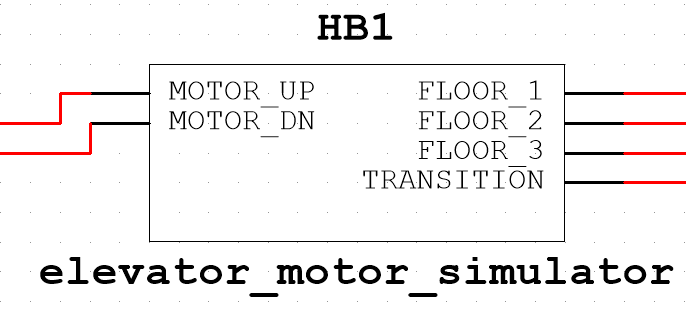
\includegraphics[width=0.6\textwidth]{elevator_motor_simulator.png}
    \caption{Black box układu symulującego silnik windy}
\end{figure}
\subsubsection{Wejścia}
\begin{itemize}
    \item \verb|MOTOR_UP| - sygnał wejściowy nakazujący poruszać się windzie w górę
    \item \verb|MOTOR_DN| - sygnał wejściowy nakazujący poruszać się windzie w dół
\end{itemize}
\subsubsection{Wyjścia}
\begin{itemize}
    \item \verb|FLOOR_1| - sygnał wyjściowy informujący o tym, że winda znajduje się na 1 piętrze,
                            aktywny w stanie wysokim
    \item \verb|FLOOR_2| - sygnał wyjściowy informujący o tym, że winda znajduje się na 2 piętrze,
                            aktywny w stanie wysokim
    \item \verb|FLOOR_3| - sygnał wyjściowy informujący o tym, że winda znajduje się na 3 piętrze,
                            aktywny w stanie wysokim
    \item \verb|TRANSITION| - sygnał wyjściowy informujący o tym że winda jest obecnie w ruchu,
                            aktywny w stanie wysokim
\end{itemize}
\subsubsection{Realizacja układu}
Do realizacji układu wykorzystaliśmy 4 bitowy licznik z biblioteki komponentów programu Multisim,
układ \verb|74LS193N|. Poniżej zamieszczamy tabelkę przedstawiającą działanie układu:
\begin{center}
    \begin{tabular}{|c|c|c|c||c|}
        \hline \verb|CLR| & \verb|~LOAD| & \verb|Up| & \verb|Down| & Mode \\
        \hline H & X & X & X & Reset(Async.) \\
        \hline L & L & X & X & Preset(Async.) \\
        \hline L & H & H & H & No Change \\
        \hline L & H & $\uparrow$ & H & Count Up \\
        \hline L & H & H & $\uparrow$ & Count Down \\
        \hline
    \end{tabular}
    \captionof{table}{Źródło: \url{https://www.multisim.com/help/components/binary-counters/}}
\end{center}
\begin{abstract}
    \begin{itemize}
        \item H - stan wysoki na wejściu
        \item L - stan niski na wejściu
        \item X - dowolny stan na wejściu
        \item $\uparrow$ - narastające zbocze sygnału
    \end{itemize}
\end{abstract}
Stworzyliśmy układ kombinacyjny, który mapuje wyjście zegara, na adres demultiplexera, który 
z kolei przekazuje jedynkę logiczną na odpowiednie wyjście. 
Przyjęliśmy, że:
\begin{itemize}
    \item 0000 - winda jest na 1 piętrze
    \item 1000 - winda jest na 2 piętrze
    \item 1111 - winda jest na 3 piętrze
    \item każdy inny - winda porusza się między piętrami
\end{itemize}
Jako demultiplexer wykorzystaliśmy układ \verb|U7A 4555BD_5V|. Jest to demultiplexer 1: 4, z 2 
bitami adresowymi.

Do wyprowadzenia formuł wykorzystaliśmy skrypt w języku Python, który generuje tabelę prawdy oraz
minimalizuje formuły logiczne. Poniżej zamieszczamy kod programu oraz wynik jego działania:
\begin{minted}[
    frame=lines,
    framesep=2mm,
    baselinestretch=1.2,
    bgcolor=LightGray,
    fontsize=\footnotesize,
    linenos
]{python}
import logicmin
elevator_motor_mux_tt = logicmin.TT(4, 2)

for i in range(16):
    permutation = bin(i).removeprefix("0b").rjust(4, '0')
    
    a1 = '1'
    b1 = '1'

    if i == 0:
        a1 = '0'
        b1 = '0'
    elif i == 8:
        a1 = '1'
        b1 = '0'
    elif i == 15:
        a1 = '0'
        b1 = '1'

    elevator_motor_mux_tt.add(permutation, [a1, b1])

print("--------------------------------elevator_motor_tt")
sols = elevator_motor_mux_tt.solve()
print(sols.printN(xnames=['QD', 'QC', 'QB', 'QA'],ynames=['1A', '1B']))
\end{minted}
Wynikiem działania skryptu są zminimializowane formuły logiczne:

\begin{verbatim}
--------------------------------elevator_motor_tt
1B <= QA + QB + QC
1A <= QD'.QA + QC'.QB + QC.QA' + QD.QB'
\end{verbatim}

Po zaimplementowaniu układu w programie Multisim, uzyskaliśmy następujący schemat:
\begin{figure}[H]
    \centering
    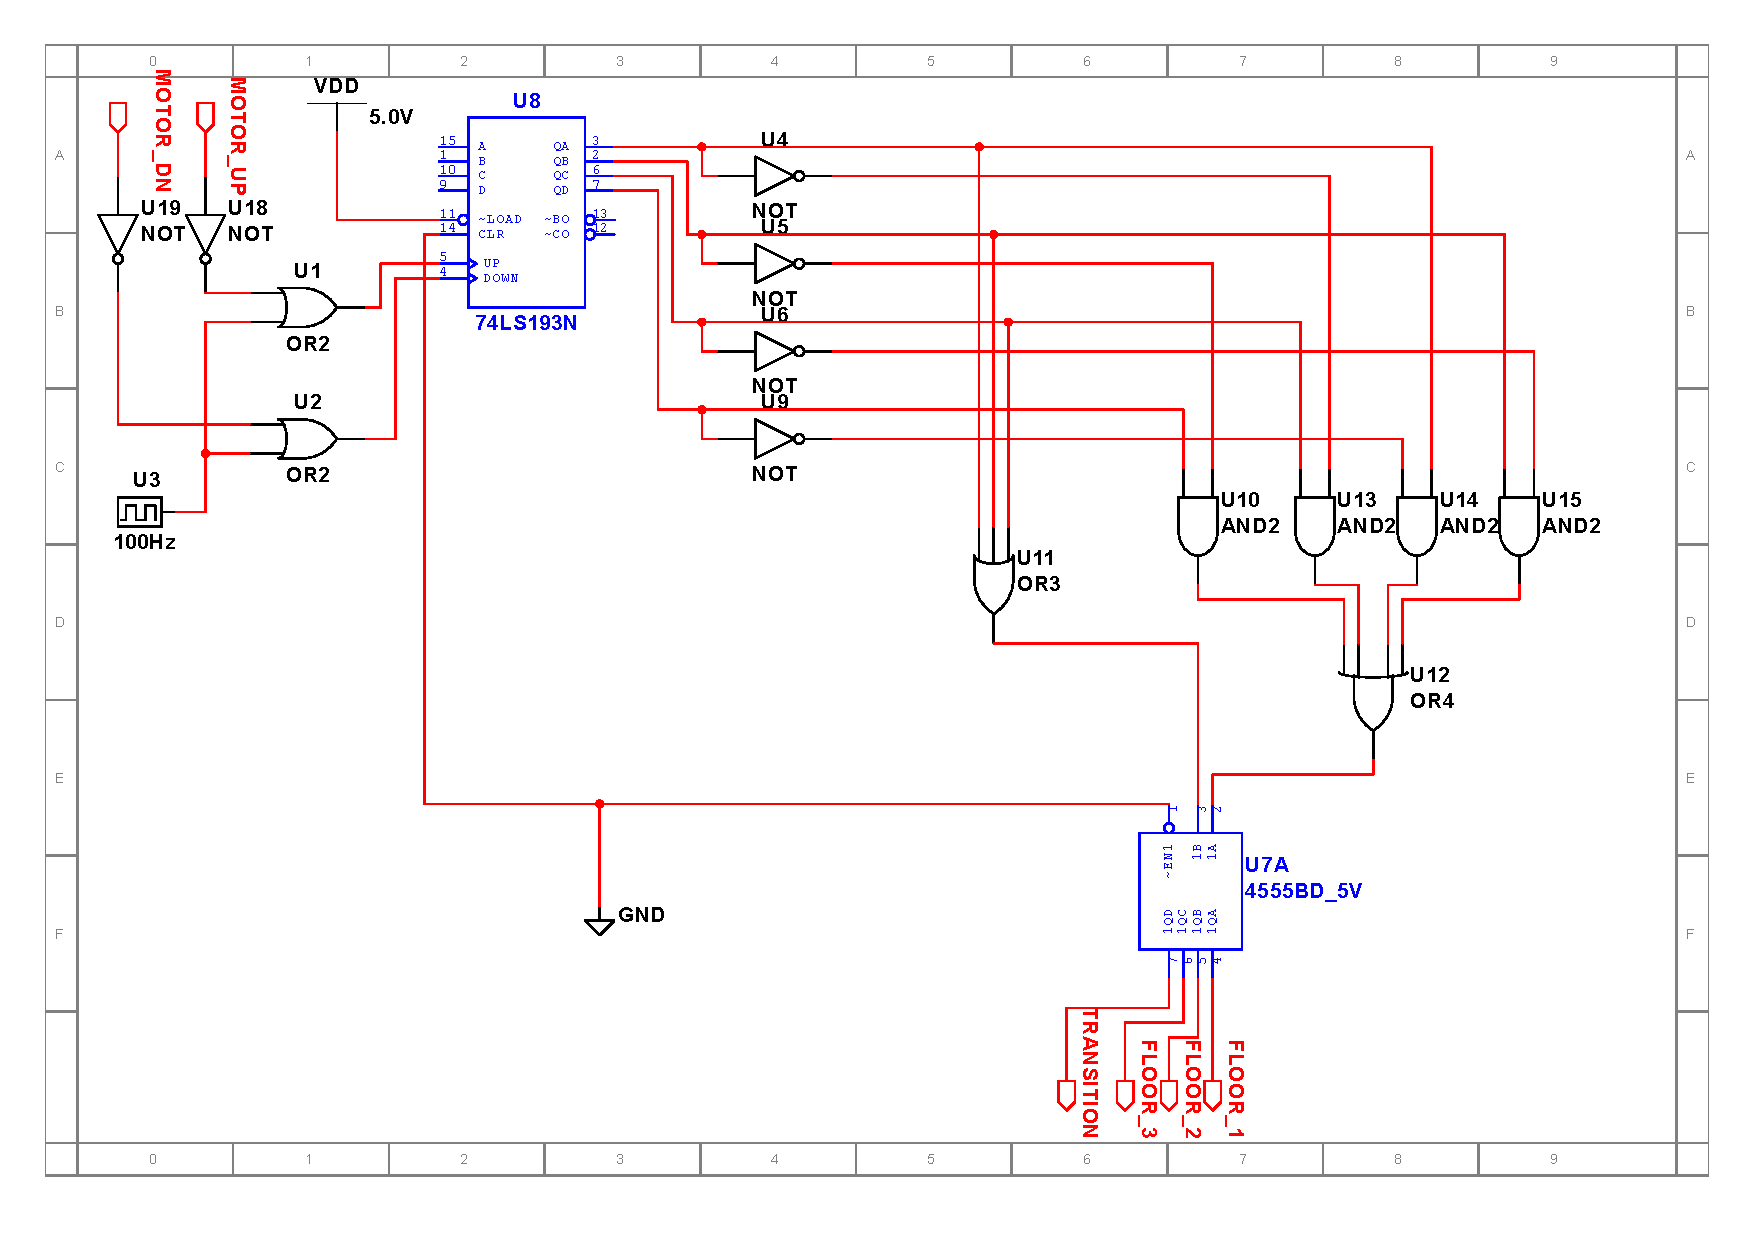
\includegraphics[width=\textwidth]{elevator_motor_simulator_schemat.pdf}
    \caption{Schemat układu symulującego silnik windy}
\end{figure}

Bramki logiczne \verb|NOT| i \verb|OR| na wejściu układu służą do przekazywania stanu wysokiego 
lub zegara na wejście licznika. Zgodnie z tabelką działania układu zapewniają one, że 
w momencie gdy chcemy liczyć do góry, układ przekazuje stan wysoki na wejście licznika \verb|DOWN|
oraz sygnał zegara na wejście licznika \verb|UP|.

\section{Testy}
\section{Zastosowania}
\section{Wnioski}

\end{document}